% $Id: ScriptedMath.tex,v 1.1 2008/01/31 18:04:17 dconway Exp $
\chapter{\label{chapter:InlineMath}Inline Mathematics in GMAT}
\chapauthor{Darrel J. Conway}{Thinking Systems, Inc.}

GMAT provides a flexible mechanism that lets users place both scalar and matrix computations into
the command sequence for a mission.  This mechanism is implemented in a set of classes described in
this chapter.

\section{Scripting GMAT Mathematics}

Mathematics in GMAT scripts follow the conventions established in MATLAB; an equation consists of an
object on the left side of an equals sign, with an equation on the right.  Equations can be entered
either in script files, or using a panel on the graphical user interface.  Parentheses are used to
set the precedence of operations when the normal precedence rules are not valid.
Table~\ref{table:operators} lists the operators implemented in GMAT. The table is arranged in order
of operator precedence; operators higher in the table are evaluated before operators that appear
lower in the table. Users can override this order through selective use of parentheses.

\begin{table}[tb]

\caption{\label{table:operators}Operators and Operator Precedence in GMAT}
\begin{tabular}{|>{\raggedright\hspace{0pt}}p{1.15in}%
                |>{\raggedright\hspace{0pt}}p{1.15in}%
                |>{\raggedright\hspace{0pt}}p{1.5in}%
                |>{\raggedright\hspace{0pt}}p{1.5in}|}
\hline
  \textbf{Operator or Function}& \textbf{Implemented Cases}&\textbf{Comments}& \textbf{Example}
\tabularnewline
\hline \hline
%  Evaluate Parameters and object& Any GMAT parameter& & sat.Earth.SMA
%\tabularnewline \hline
  Evaluate Conversion Functions& DegToRad, RadToDeg& Converts between radians and
degrees&DegToRad(sat.RAAN)
\tabularnewline \hline
  Evaluate Matrix Operations& transpose and ', det, inv and \textasciicircum{}(-1), norm& & mat',
det(mat)
\tabularnewline \hline
  Evaluate Math Functions& sin, cos, tan, asin, acos, atan, atan2, log, log10, exp, sqrt& Angles in
the trig functions are in radians& sin(DegToRad(sat.TA))
\tabularnewline \hline
  Exponentiation&\textasciicircum{}& Powers are any real number& sin(radTA)\textasciicircum{}0.5
\tabularnewline \hline
  Multiplication and Division& {*} /& & sat.RMAG / sat.SMA
\tabularnewline \hline
  Addition and Subtraction& + -& & sat.RAAN + sat.AOP
\tabularnewline \hline
\end{tabular}
\end{table}

Mathematics in GMAT are scripted using the same syntax as assignments.  Three
samples of the scripting for the operations in Table~\ref{table:operators} are
provided here to and discussed in the design presentation to help explain how
GMAT manipulates its internal data structures to perform scripted mathematics.

\subsection*{Example 1: Basic Arithmetic}
In this simplest example, a user needs to write script to perform the
calculation of the longitude of periapsis,

\begin{equation}\label{eq:mathLongPeri}
\Pi=\Omega+\omega
\end{equation}

\noindent for the spacecraft named sat.  The scripting for this calculation is
straight forward:

\begin{quote}
\begin{verbatim}
Create Spacecraft sat;
Create Variable arg
GMAT arg = sat.RAAN + sat.AOP
\end{verbatim}
\end{quote}

\subsection*{Example 2: More Complicated Expressions}

This snippet calculates the separation between two spacecraft, using the
Pythagorean theorem:

\begin{equation}\label{eq:mathSatSep}
\Delta R = \sqrt{(X_1 - X_2)^2 + (Y_1 - Y_2)^2 + (Z_1 - Z_2)^2}
\end{equation}

\noindent This is a useful example because, as we will see, it exercises the
parser to ensure that operations are performed in the correct order.  The
script for this example is, again, pretty simple:

\begin{quote}
\begin{verbatim}
Create Spacecraft sat1, sat2;
Create Variable sep
GMAT sep = sqrt((sat1.X-sat2.X)^2 + (sat1.Y-sat2.Y)^2 + (sat1.Z-sat2.Z)^2)
\end{verbatim}
\end{quote}

\subsection*{Example 3: Matrix Computations}

This final example is more complex, and exercises both operator ordering and
matrix computations to calculate a component of the analytic gradient of a
function used in optimization.  This script snippet assumes that GMAT can
calculate the State Transition Matrix and provide users with access to the
corresponding 3x3 submatrices of it.  The scripting for that calculation is:

\begin{quote}
\begin{verbatim}
% This script snippet uses the following definitions for pieces of the
% State Transition Matrix (STM):
%    Sat.Phi is a 6x6 matrix that is the spacecraft STM
%    Sat.PhiA is the upper left 3x3 portion of the STM
%    Sat.PhiB is the upper right 3x3 portion of the STM
%    Sat.PhiC is the lower left 3x3 portion of the STM
%    Sat.PhiD is the lower right 3x3 portion of the STM

Create Spacecraft Sat1, Sat2
Create Array Svec[3,1] Svecdot[3,1] S[1,1] dSdotdR[1,3]

For I = 1: 100
   % Step the spacecraft
   Propagate LowEarthProp(Sat1,Sat2);

   % Calculate the relative position and velocity vectors
   GMAT Svec(1,1) = Sat2.X - Sat1.X;
   GMAT Svec(2,1) = Sat2.Y - Sat1.Y;
   GMAT Svec(3,1) = Sat2.Z - Sat1.Z;
   GMAT Svecdot(1,1) = Sat2.VX - Sat1.VX;
   GMAT Svecdot(2,1) = Sat2.VY - Sat1.VY;
   GMAT Svecdot(3,1) = Sat2.VZ - Sat1.VZ;

   % Calculate range
   GMAT S =  norm(Svec);

   % Calculate the change in the range rate due to a change in the
   % initial position of sat1
   GMAT dSdotdR = 1/S*( Svecdot' - Svec'*Svecdot*Svec'/S^2 )*(- Sat1.PhiA )...
                  + Svec'/S*(-Sat1.PhiC);
EndFor;
\end{verbatim}
\end{quote}

\noindent The last expression here, dsDotdR, will be used in the design
discussion.

\section{Design Overview}

When GMAT encounters the last line of the first script snippet:

\begin{quote}\begin{verbatim}
GMAT arg = sat.RAAN + sat.AOP
\end{verbatim}\end{quote}

\noindent it creates an assignment command that assigns the results of a calculation to the variable
named arg. The right side of this expression -- the equation -- is converted into GMAT objects using
an internal class in GMAT called the MathParser.  The MathParser sets up custom calculations by
breaking expressions -- like the ones scripted in the preceding section -- into a tree structure
using a recursive descent algorithm.  This decomposition is performed during script parsing when the
user is running from a script file, and during application of user interface updates if the user is
constructing the mathematics from the GMAT graphical user interface.  GMAT stores the tree
representation of the mathematics in an internal object called the MathTree.  During script
execution, the MathTree is populated with the objects used in the calculation during mission
initialization in the Sandbox.  The equation is evaluated when the associated Assignment command is
executed by performing a depth-first traversal of the tree to obtain the desired results.  The
algorithms implemented here are extensions of the approach presented in chapter 40 of
\cite{schildt}.

\begin{figure}[tb]
\begin{center}
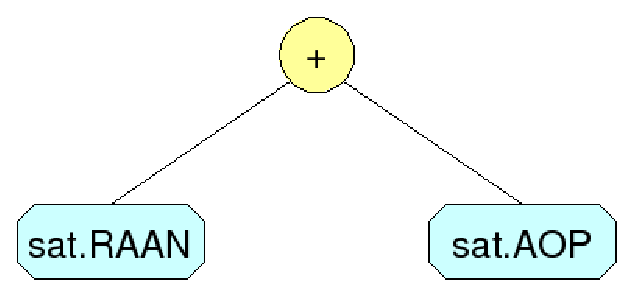
\includegraphics[scale=0.5]{Images/nodePlusAop.eps}
\caption{\label{figure:longPeriapseTree}Tree View of the Longitude of Periapsis Calculation}
\end{center}
\end{figure}

The tree based structure of the computations enforces the operator precedence rules tabulated above.
 In this section the construction and evaluation of the trees for the examples is presented, and the
classes used in this process are introduced.  The sections that follow this overview present the
classes in a more systematic manner, discuss how the scripting is parsed to create the GMAT objects
used in evaluation, and then tie these pieces together by discussing how the constructed objects
interact as a program executes.

Figure~\ref{figure:longPeriapseTree}\footnote{In this figure and those that follow, the components
that can be evaluated into Real numbers are drawn on elongated octagons, and the operators are drawn
in a circle or ellipse.  Matrices are denoted by a three-dimensional box.  Empty nodes are denoted
by black circles, and numbers, by orange squares with rounded corners.} shows the tree generated for
the longitude of periapsis calculation scripted above.  This simplest example illustrates the layout
of the tree in memory that results from a simple arithmetic expression. The GMAT MathParser class is
fed the right side of the expression from the script -- in this case, that is the string "sat.RAAN +
sat.AOP".  This string is passed to the recursive descent code, which breaks it into three pieces --
two expressions that can be evaluated directly, and an operator that combines these expressions. 
These pieces are stored in an internal class in GMAT called the MathTree.  The expressions
"sat.RAAN" and "sat.AOP" are placed into the "leaves" of the tree, while the addition operator is
placed in the top, "internal" node.  The leaf nodes are all instances of a class named
"MathElement", and the internal nodes, of classes derived from a class named "MathFunction".  When
the assignment command containing this construct is executed, each of the leaves of the tree is
evaluated, and then combined using the code for the addition operator.

\begin{figure}[tb]
\begin{center}
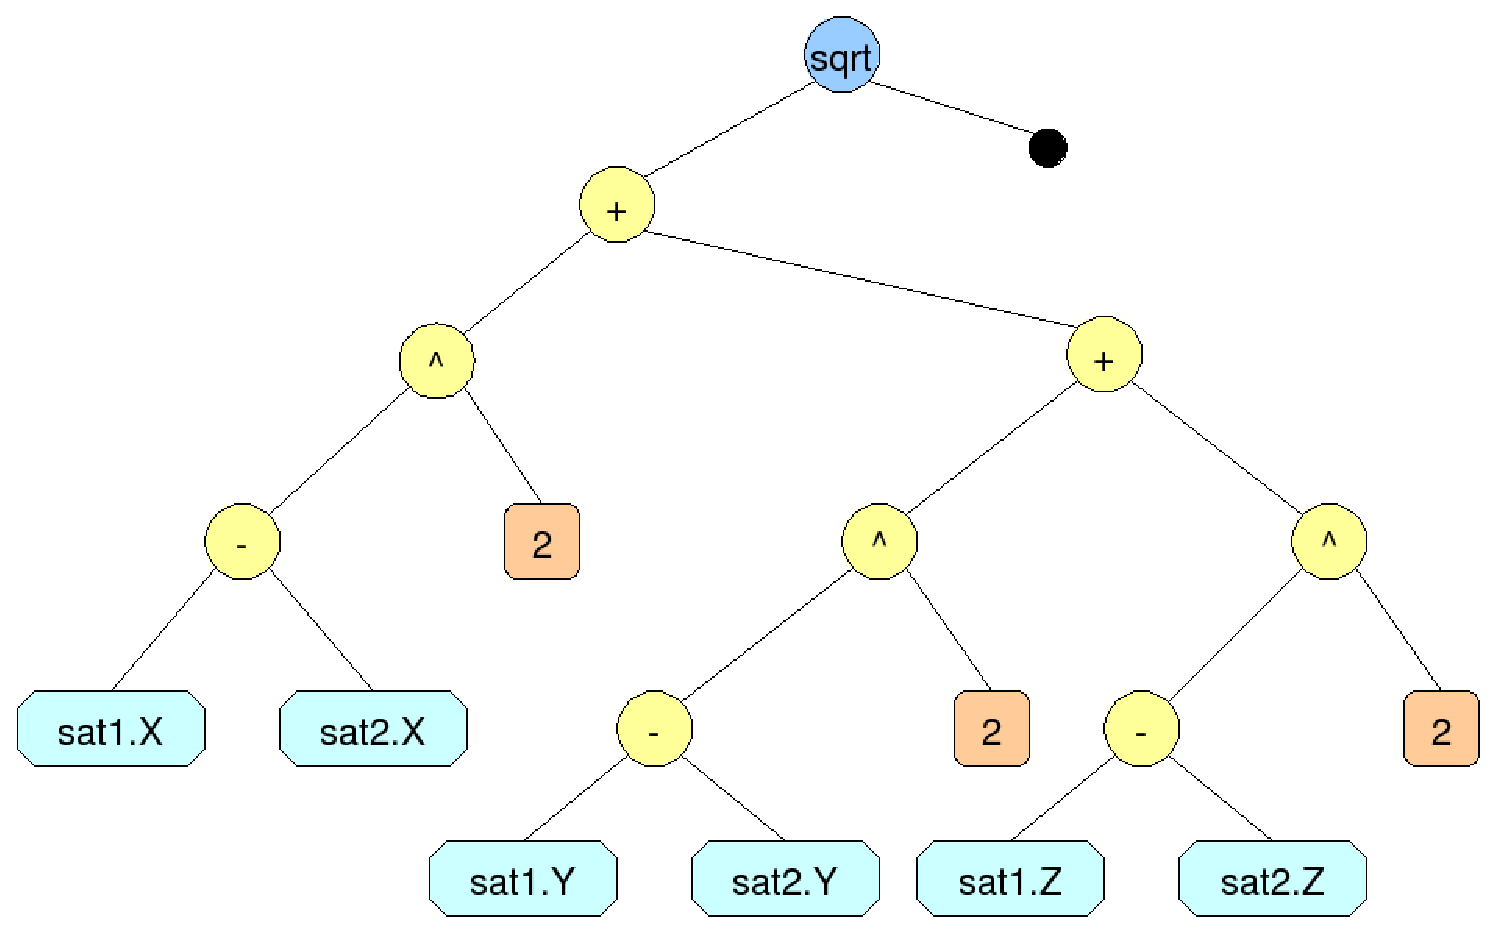
\includegraphics[scale=0.5]{Images/satSep.eps}
\caption{\label{figure:satelliteSeparationTree}Tree View of the Satellite
Separation Calculation}
\end{center}
\end{figure}

The second example, illustrated in Figure~\ref{figure:satelliteSeparationTree},
provides a more illustrative example of the parsing and evaluation algorithms
implemented in GMAT.  This tree illustrates the equation encoded in example 2:

\begin{quote}\begin{verbatim}
GMAT sep = sqrt((sat1.X-sat2.X)^2 + (sat1.Y-sat2.Y)^2 + (sat1.Z-sat2.Z)^2)
\end{verbatim}\end{quote}

\noindent Each node in the MathTree can be one of three types: a
function node, an operator node (both of these types are embodied in the
MathFunction class), or an element node (in the MathElement class).  The
element nodes are restricted to being the leaf nodes of the tree; the internal
nodes are all either function nodes or operator nodes.

Each MathElement node consists of two separate pieces; a string containing the
text of the expression represented by the node, and either a pointer to the
object that embodies that expression or, for constants, a local member
containing the value of the expression.  The pointer member is initially set to NULL when the
MathElement node is constructed during script parsing.  When the
script is initialized in the GMAT Sandbox, these pointers are set to the
corresponding objects in the Sandbox's configuration.  Each time the assignment command associated
with the MathTree executes, an Evaluate() method is called
on the MathTree, as described below.

The function and operator nodes consist of several pieces as well.  Each of
these nodes contain subnode pointers that identify the input value or values
needed for the node evaluation, and a method that performs the actual
mathematics involved in the evaluation.  The mathematical operations for each
of these nodes is coded to work on either a scalar value or a matrix; the
specific rules of implementation are operator specific.

The Evaluate() method for the MathTree calls the Evaluate() method for the
topmost node of the tree.  This method call is evaluated recursively for all of the subnodes of the
tree, starting at the top node.  The method checks to see
if the node is a leaf node or an internal node.  If it is a leaf node, it is
evaluated and the resulting value is returned to the object that called it.  If it is an internal
node, it evaluates its subnodes by calling Evaluate() first
on the left node, then on the right node.  Once these results are obtained,
they are combined using the mathematical algorithm coded for the node, and the
resulting value is then returned to the calling object.

\begin{figure}[tb]
\begin{center}
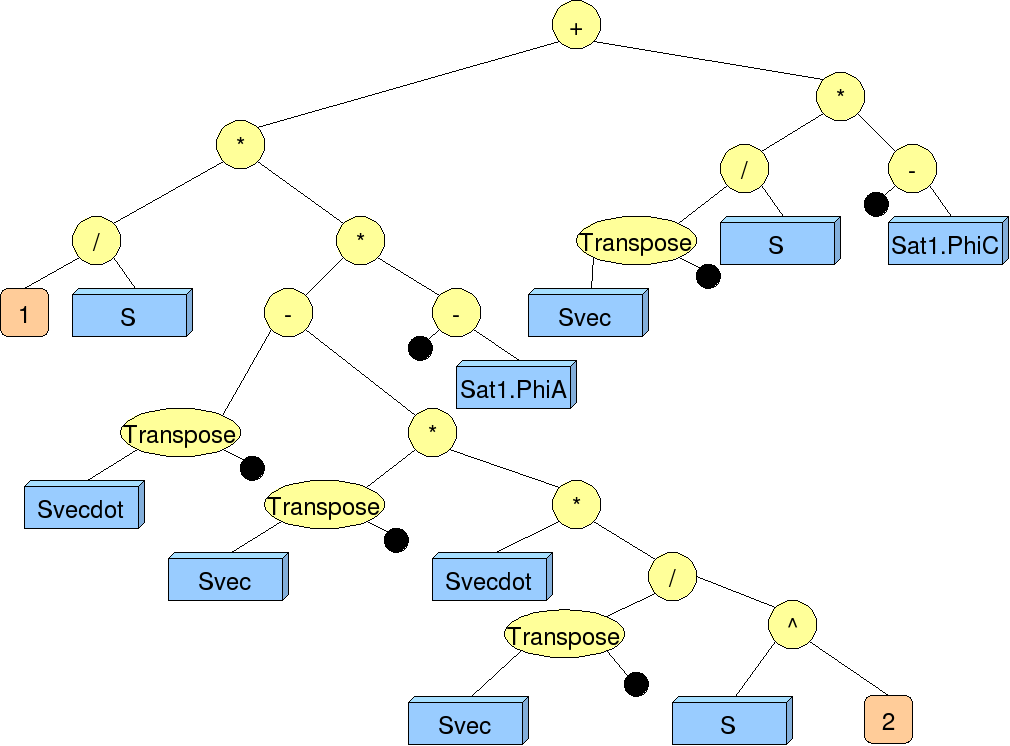
\includegraphics[scale=0.5]{Images/MatrixExample.eps}
\caption{\label{figure:matrixMathTree}Tree View of the Matrix Calculation in
Example 3}
\end{center}
\end{figure}

Finally, the gradient component scripted in the third example:

\begin{quote}\begin{verbatim}
GMAT dSdotdR = 1/S*( Svecdot' - Svec'*Svecdot*Svec'/S^2 )*(- Sat1.PhiA )...
               + Svec'/S*(-Sat1.PhiC);
\end{verbatim}\end{quote}

\noindent produces Figure~\ref{figure:matrixMathTree}.  Evaluation for this tree proceeds as
outlined above, with a few variations.  Instead of calling the Evaluate() method for the nodes in
the tree, expressions that use matrices call the MatrixEvaluate method.  Another wrinkle introduced
by the matrix nature of this example is that the internal nodes now have an additional requirement;
each node needs to determine that the dimensionality of the subnodes is consistent with the
requested operations.  This consistency check is performed during initialization in the Sandbox,
using the ValidateInputs() method.
MatrixEvaluate may perform additional checks during execution, so that
singularities in the computation can be flagged and brought to the attention of the user.

\section{Core Classes}

\begin{figure}
\begin{center}
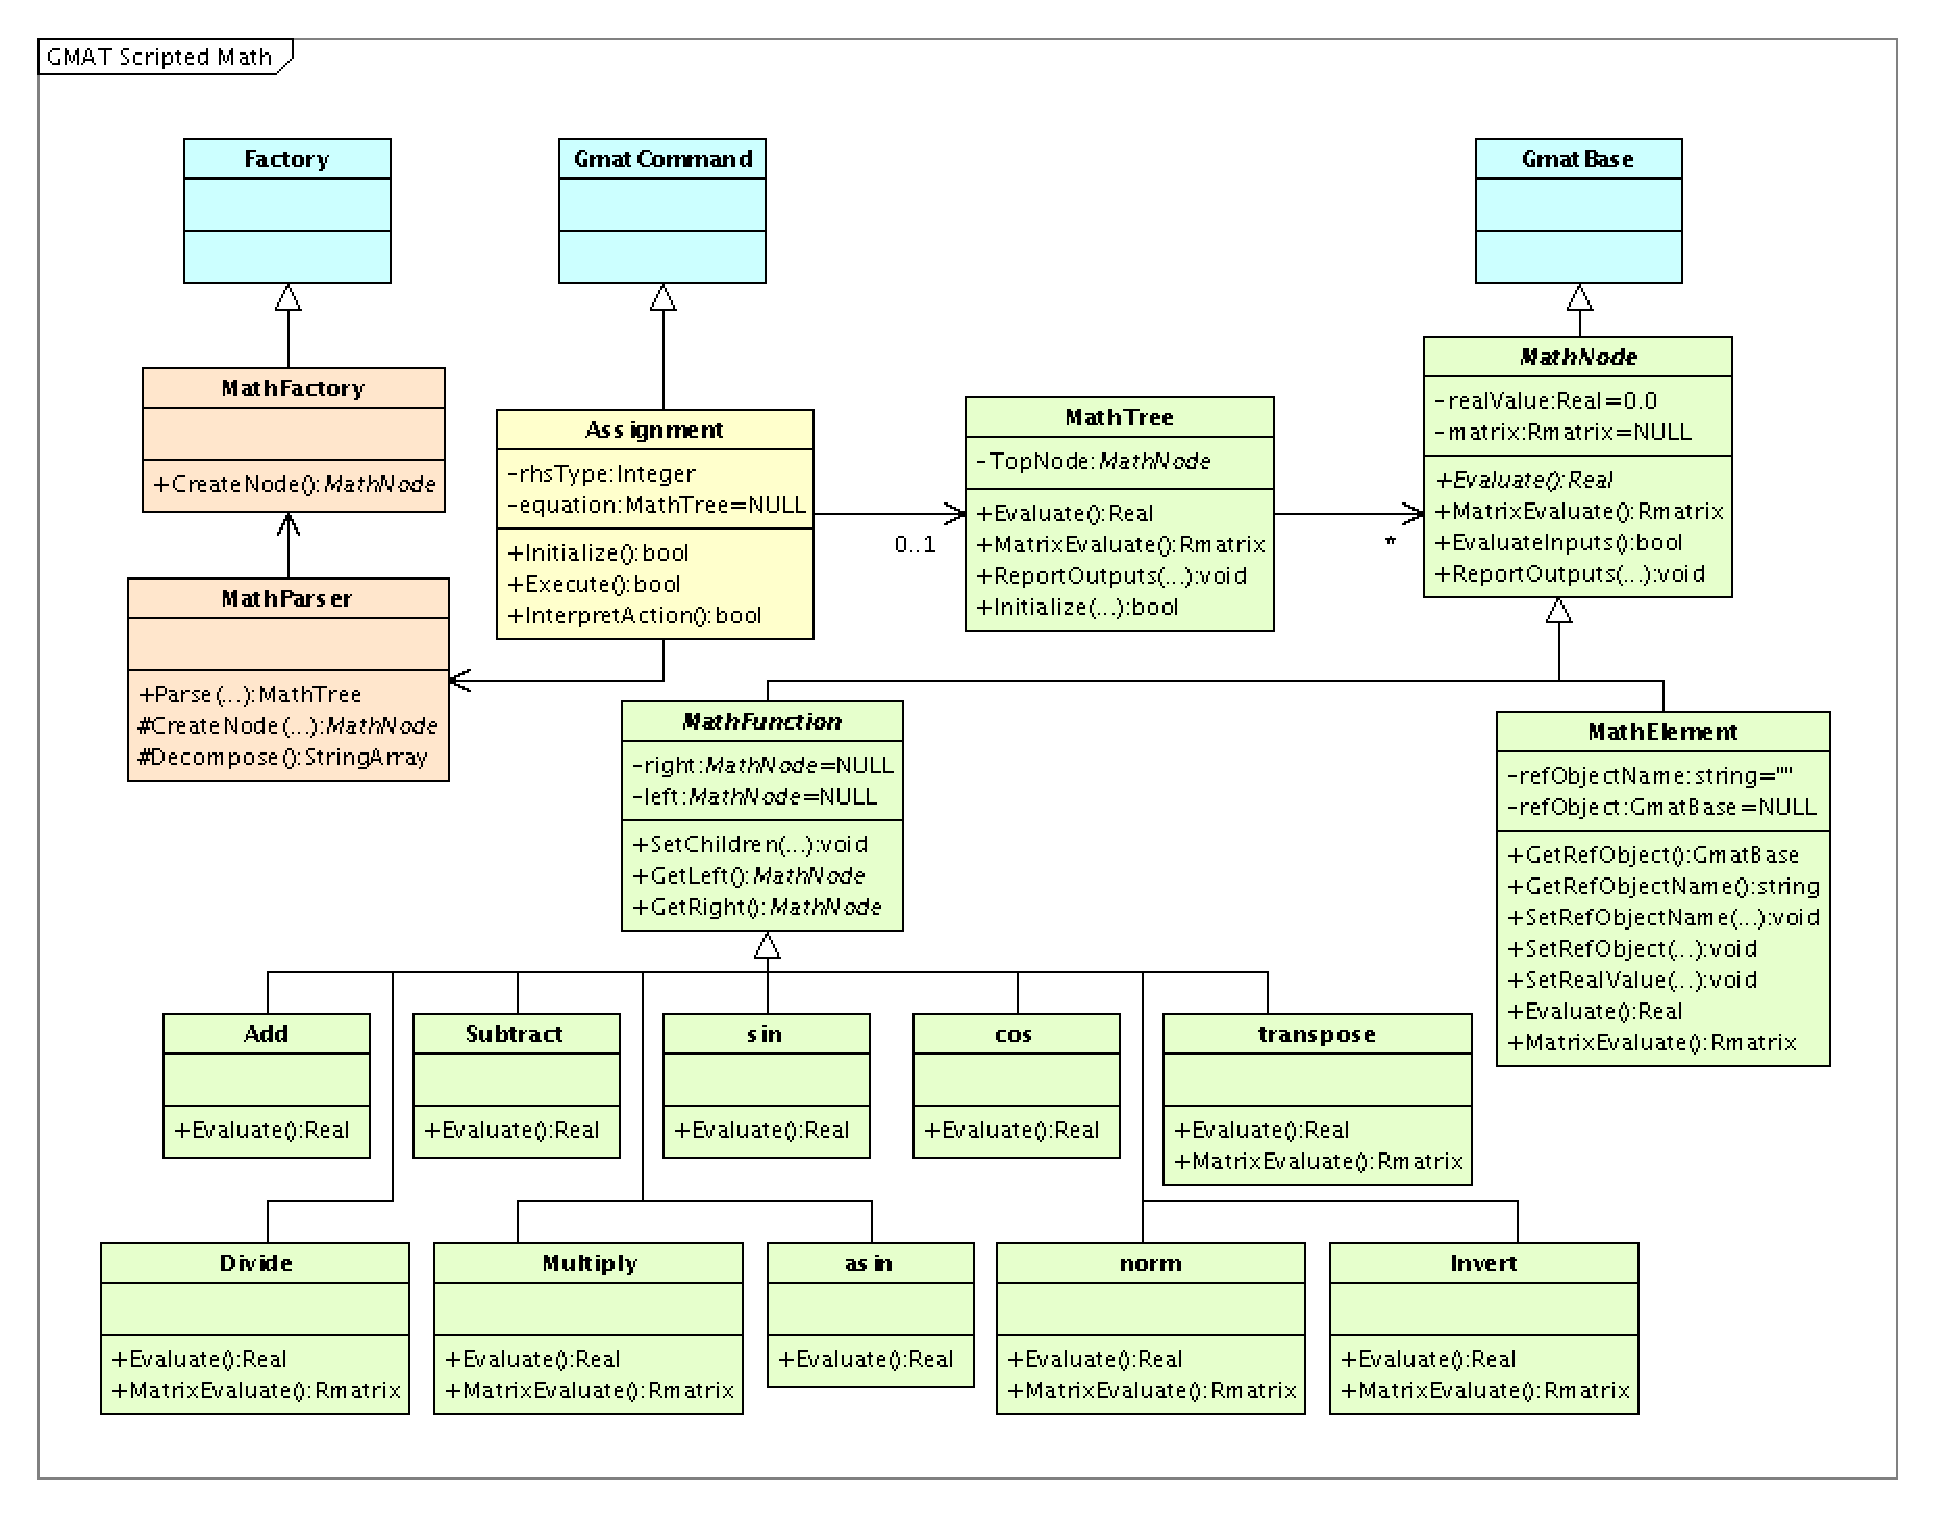
\includegraphics[scale=0.5]{Images/MathClasses.eps}
\caption{\label{figure:MathClasses}Classes Used to Implement GMAT Mathematics}
\end{center}
\end{figure}

Figure~\ref{figure:MathClasses} shows the class hierarchy implemented to
perform the operations described above, along with some of the core members of
these classes.  The core classes used in GMAT to perform mathematical
operations are shown in green in this figure, while the helper classes used to
setup the binary tree structure are shown in orange.  The MathTree and its
nodes are all owned by instances of the Assignment command, shown in yellow in
the figure.  Core GMAT classes are shaded in blue.  The main features of these
classes are shown here, and discussed in the following paragraphs.  At the end
of this section, the principal elements of the base classes are collected for
reference.

The MathTree class is the container for the tree describing the equation.  It
contains a pointer to the topmost node of the tree, along with methods used to
manipulate the tree during initialization and execution.  This class is used to provide the
interface between the tree and the Assignment command.

Each node in a MathTree is derived from the MathNode class.  That base class
provides the structures and methods required by the MathTree to perform its
functions.  There are two classes derived from the MathNode base: MathElement
and MathFunction.  The MathElement class is used for leaf nodes, and can store
either a numerical value, a matrix, or a GMAT object that evaluates to a
floating point number -- for example, a Parameter, or a real member of a core
GMAT object.  MathFunction instances are used to implement mathematical
operators and functions.  The left and right subnodes of these nodes contain
the function or operator operands.  Subnodes are evaluated before the operator
is evaluated, producing results that are used when evaluating the function.

The MathNode base class contains two members that are used to check the
compatibility of operands during initialization.  The EvaluateInputs() method
checks the return dimensions of the subnodes of the node, and returns true if
either the node is a MathElement or if the subnodes are compatible with the
current node's Evaluate() and MatrixEvaluate() methods.  The ReportOutputs()
method is called on subnodes to obtain the dimensions of matrices returned from calls to
MatrixEvaluate().  That method provides an interface used by the
EvaluateInputs() method to perform its evaluation.

One additional item worth mentioning in the MathNode base class is the
implementation of the MatrixEvaluate() method.  The Evaluate() method is pure
virtual, and therefore not implemented in the base class.  MatrixEvaluate(), on the other hand, is
implemented to apply the Evaluate() method element by
element to the matrix members.  In other words, the default MatrixEvaluate()
method implements the algorithm

\begin{equation}\label{eq:mathDefaultMatrixCalc}
M_{ij} = Op(L_{ij},R_{ij})
\end{equation}

\noindent where $M_{ij}$ is the [i,j] element of the resultant, $L_{ij}$ is the
[i,j] element of the left operand, and $R_{ij}$ is the [i,j] element of the
right operand.  Most classes derived from the MathFunction class will override
this implementation.

The classes implementing mathematical operations are derived from the MathFunction class.
Figure~\ref{figure:MathClasses} shows some (but not all) of these derived classes.  Operators that
have a one to one functional correspondence with MATLAB operations are named identically to the
MATLAB function.  That means that operators like the transpose operator will violate the GMAT naming
conventions, at least for the string name assigned to the class, because the MATLAB operator is
lowercase, ``transpose'', while the GMAT naming convention specified that class names start with an
upper case letter.

Operations that can rely on the algorithm presented in equation~\ref{eq:mathDefaultMatrixCalc} do
not need to implement the MatrixEvaluate() method; for the classes shown here, that means that Add,
Subtract, sin, cos, and asin only need to implement the Evaluate() method, while Multiply, Divide,
transpose, norm and Invert need to implement both the Evaluate() and MatrixEvaluate() methods.

\subsection{MathTree and MathNode Class Hierarchy Summary}

This section describes the top level classes in the MathTree subsystem, summarizing key features and
providing additional information about the class members.

\subsubsection{MathTree}

A MathTree object is a container class used to help initialize and manage the tree representing an
equation.  It standardizes the interface with the Assignment command and acts as the entry point for
the evaluation of an equation.  It is also instrumental in setting the object pointers on the tree
during initialization in the Sandbox.  Key members of this class are described below.

\subparagraph{\textit{Class Attributes}}
\begin{itemize}
\item \textbf{topNode}: A pointer to the topmost node in the MathTree.
\end{itemize}

\subparagraph{\textit{Methods}}
\begin{itemize}
\item \textbf{Evaluate()}: Calls the Evaluate() method on the topNode and returns the value obtained
from that call.
\item \textbf{MatrixEvaluate()}: Calls the MatrixEvaluate() method on the topNode and returns the
matrix obtained from that call.
\item \textbf{ReportOutputs(Integer \&type, Integer \&rowCount, Integer \&colCount)}:  Calls
ReportOutputs(...) on the topNode and returns the data obtained in that call, so that the Assignment
command can validate that the returned data is compatible with the object that receives the
calculated data (i.e. the object on the left side of the equation).
\item \textbf{Initialize(std::map<std::string,GmatBase*> *objectMap)}: Initializes the data members
in the MathTree by walking through the tree and setting all of the object pointers in the
MathElement nodes.
\end{itemize}

\subsubsection{MathNode}

MathNode is the base class for the nodes in a MathTree.  Each MathNode supports methods used to
determine the return value from the node, either as a single Real number or as a matrix.  The
MathNodes also provide methods used to test the validity of the calculation contained in the node
and any subnodes that may exist.  The core MathNode members are listed below.

\subparagraph{\textit{Class Attributes}}
\begin{itemize}
\item \textbf{realValue}: Used to store the most recent value calculated for the node.
\item \textbf{matrix}: Used to store the most recent matrix data calculated for the node, when the
node is used for matrix calculations.
\end{itemize}

\subparagraph{\textit{Methods}}
\begin{itemize}
\item \textbf{Evaluate()}: An abstract method that returns the value of the node.  For MathElements,
this method returns the current value of the element, either by evaluating a Parameter and returning
the value, accessing and returning an object's internal data, or returning a constant.  For
MathFunctions, the Evaluate() method appies the function and returns the result.  If the encoded
function cannot return a Real number, Evaluate() throws an exception.
\item \textbf{MatrixEvaluate()}: Fills in a matrix with the requested data.  For MathFunction
objects, this method performs the calculation of the operation and fills in the matrix with the
results.  The default implementation uses equation~\ref{eq:mathDefaultMatrixCalc} to fill in the
matrix element by element.  Operations that do not return matrix values, like norm and determinant,
throw exceptions when this method is called.  MathElements simply return the matrix associated with
the node.
\item \textbf{EvaluateInputs()}: Checks the inputs to the node to be sure that they are compatible
with the calculation that is being performed.  For MathElement nodes, this method always returns
true if the node was successfully initialized.  For MathFunction nodes, this method calls its
subnodes and checks to be sure that the subnodes return compatible data for the function.
\item \textbf{ReportOutputs(Integer \&type, Integer \&rowCount, Integer \&colCount)}:  This method
tells the calling object the type and size of the calculation that is going to be performed by
setting values of the parameters used in the call.  The first parameter, `type', is set to indicate
whether the return value will be a matrix or a Real number.  `rowCount' and `colCount' are set to
the dimensions of the matrix if the return value is a matrix, or to 0 if the return value is scalar.
 This method is used in the EvaluateInputs() method to determine the suitability of subnodes for a
given calculation, and by the MathTree class to obtain the size of the answer returned from a
complete calculation.
\end{itemize}

\subsubsection{MathElements}

The leaf nodes of a MathTree are all instances of the MathElement class.  The MathElement class acts
as a wrapper for GMAT objects, using the methods defined in the GmatBase base class to set these
referenced objects up for the MathElement's use.  The GmatBase methods SetRefObject(),
SetRefObjectName(), GetRefObject(), and GetRefObjectName() are overridden to set the internal data
structures in the node.  The other relevant members of this class are listed below.

\subparagraph{\textit{Class Attributes}}
\begin{itemize}
\item \textbf{refObjectName}: Holds the name of the GMAT object that is accessed by this node.
\item \textbf{refObject}: A pointer to the referenced object.  This pointer is set when the MathTree
is initialized in the Sandbox.
\end{itemize}

\subparagraph{\textit{Methods}}
\begin{itemize}
\item \textbf{SetRealValue(Real value)}: Sets the value of the node when it contains a constant.
\end{itemize}

\subsubsection{MathFunctions}

The internal nodes of a MathTree are all instances of classes derived from MathFunction.  This class
contains pointers to subnodes in the tree which are used to walk through the tree structure during
initialization and evaluation.  The relevant members ate described below.

\subparagraph{\textit{Class Attributes}}
\begin{itemize}
\item \textbf{left}: A pointer to the left subnode used in the calculation.  MathFunctions that only
require a right subnode leave this pointer in its default, NULL setting.
\item \textbf{right}: A pointer to the right subnode used in the calculation.  MathFunctions that
only require a left subnode leave this pointer in its default, NULL setting.
\end{itemize}

\subparagraph{\textit{Methods}}
\begin{itemize}
\item \textbf{SetChildren(MathNode *leftChild, MathNode *rightChild)}: Sets the pointers for the
left and right child nodes.  If a node is not going to be set, the corresponding parameter in the
call is set to NULL.
\item \textbf{GetLeft()}: Returns the pointer to the left node.
\item \textbf{GetRight()}: Returns the pointer to the right node.
\item \textbf{Evaluate()}: In derived classes, this method is overridden to perform the mathematical
operation represented by this node.
\item \textbf{MatrixEvaluate()}: In derived classes that do not use the default matrix calculations
(equation~\ref{eq:mathDefaultMatrixCalc}), this method is overridden to perform the mathematical
operation represented by this node.
\end{itemize}

\subsection{Helper Classes}

There are two classes that help configure a MathTree: MathParser and MathFactory.  In addition, the
Assignment command acts as the interface between a MathTree and other objects in GMAT, and the
Moderator provides the object interfaces used to configure the tree.  This section sketches the
actions taken by these components.

\subsubsection{MathParser}

The Interpreter subsystem (see Section~\ref{section:InterpreterOverview}) in GMAT includes an
interface that can be used to obtain a MathParser object.  This object takes the right side of an
equation, obtained from either the GMAT GUI or the ScriptInterpreter, and breaks it into a tree
that, when evaluated depth first, implements the equation represented by the equation.  The
MathParser uses the methods described below to perform this task.

\subparagraph{\textit{Methods}}
\begin{itemize}
\item \textbf{Parse(const std::string \&theEquation)}: Breaks apart the text representation of an
equation and uses the component pieces to construct the MathTree.
\item \textbf{CreateNode(const std::string \&genString)}: Uses the generating string ``genString'',
to create a node for insertion into the MathTree.
\item \textbf{Decompose(const std::string \&composite)}: This method is the entry point to the
recursive descent algorithm.  It uses internal methods to take a string representing the right side
of the equation and break it into the constituent nodes in the MathTree.  The method returns the
topmost node of the MathTree, configured with all of the derived subnodes.
\end{itemize}

\subsubsection{MathFactory}

The MathFactory is a GMAT factory (see Chapter~\ref{chapter:Factories} that is used to construct
MathNodes.  It has one method of interest here:

\subparagraph{\textit{Methods}}
\begin{itemize}
\item \textbf{CreateNode(const std::string \&ofType)}: Creates a MathNode that implements the
operation contained in the string.  If no such operator exists, the MathFactory creates a
MathElement node and sets the reference object name on that node to the test of the `ofType' string.
\end{itemize}

\subsubsection{The Assignment Command and the Moderator}

The Assignment command is the container for the MathTree described in this chapter.  All GMAT
equations are formatted with a receiving object on the left side of an equals sign, then the equals
sign, and then the equation on the right.  When the interpreter system is configuring an Assignment
command, it detects when the right side is an equation, and passes the string describing the
equation into a MathParser.  That MathParser proceeds to parse the equation, making calls into the
Moderator when a new MathNode is required.  The Moderator accesses the MathFactories through the
FactoryManager, and obtains MathNodes as required.  These nodes are not added to the Configuration
Manager, but they are returned to the MathParser for insertion into the current MathTree.  Once the
tree is fully populated, it is returned to the Assignment command, completing the parsing of the
expression.

When the Moderator is instructed to run a mission, it passes the configured objects into the
Sandbox, and then initializes the Sandbox.  The last step in Sandbox initialization is to initialize
all of the commands in the mission sequence.  When one of these commands is an Assignment command
that includes a MathTree, that command initializes the MathTree after initializing all of its other
elements, and then validates that the MathTree is compatible with the object on the left side of the
equation.  If an error is encountered at this phase, the Assignment command throws an exception that
describes the error and includes the text of the command that failed initialization.  If
initialization succeeds, the Moderator then tells the Sandbox to run the mission.  The Sandbox
starts at the first command in the mission sequence, and executes the command stream as described in
Chapter~\ref{chapter:Commands}.

\section{Building the MathTree}

\begin{figure}
\begin{center}
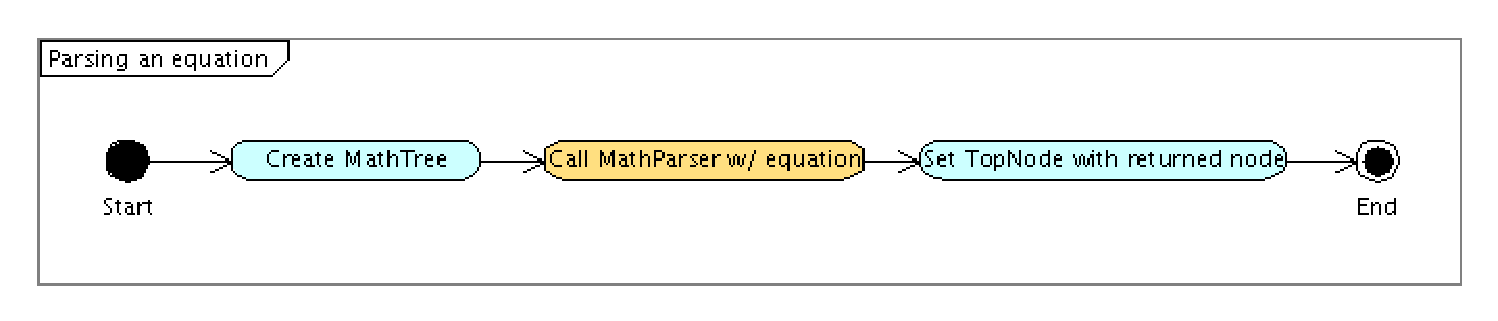
\includegraphics[scale=0.5]{Images/MathParserTop.eps}
\caption{\label{figure:MathParserTop}Control Flow for Parsing an Equation}
\end{center}
\end{figure}

Scripted mathematics are constructed using the MathParser class, which builds
the binary tree representing the equation that is evaluated by constructing
nodes for the tree and placing these nodes into the tree one at a time.
Figure~\ref{figure:MathParserTop} shows the high level control flow used to
create the MathTree.  An empty MathTree is created, and then that tree is
passed into the MathParser along with the string representation of the
equation.  The Mathparser takes the MathTree and populates it with MathNodes
based on the equation string.  The top node of this completed tree is then
returned from the parser, and set on the assignment command for use during
execution of the mission.

\begin{figure}
\begin{center}
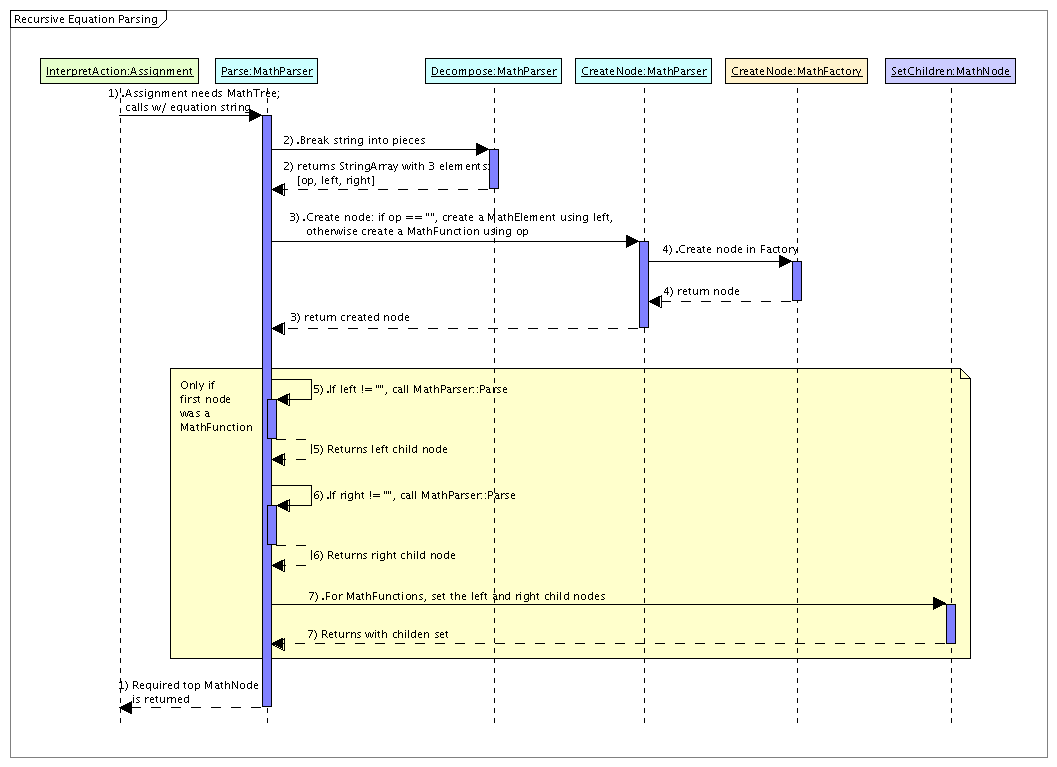
\includegraphics[scale=0.4]{Images/ParseRecursion.eps}
\caption{\label{figure:ParserRecursion}Parser Recursion Sequence}
\end{center}
\end{figure}

The middle step in the process outlined in Figure~\ref{figure:MathParserTop}
encapsulates the recursive descent decomposition of the equation.
Figure~\ref{figure:ParserRecursion} provides a more detailed view of this
algorithm.  The InterpretAction method of the Assignment command determines
that the right side of the assignment is an equation, and then creates a
MathTree and a MathParser to break this equation into the components needed for evaluation during
execution.  The MathTree and the equation string are passed
into the MathParser.

The MathParser takes the input string, and attempts to break it into three
pieces: an operator, a left element, and a right element.  Any of these three
pieces can be the empty string; if the operator string is empty, only the left
string contains data, denoting that the string is used to build a MathElement
node, on one of the leaves of the MathTree.

If the operator string is not empty, the operator string is used to build a
MathFunction node.  MathFunction nodes are used to perform all mathematical
operations: basic math like addition, subtraction, multiplication, division,
and exponentiation, along with unary negation and mathematical functions.  The
arguments of the MathFunction are contained in the left and right strings.
These strings are passed into the MathParser's Parse method for further
decomposition, and the process repeats until all of the strings have been
decomposed into operators and the MathElement leaf nodes.  If either string is
empty, the corresponding child node on the MathFunction is set to NULL.

Once a leaf node has been constructed, that node is set as the left or right
node on the operator above it.  Once the left and right nodes are set on a
MathFunction, that node is returned as a completed node to the calling method,
terminating that branch of the recursion.  When the topmost node has its child
nodes filled in, the MathParser returns from the recursion with the completed
MathTree.

\section{Program Flow and Class Interactions}

The preceding section describes the construction of the MathTree that
represents an equation. The parsing described above places the instances of the
MathFunction nodes into the MathTree, along with the string names of the
MathElement nodes.  The objects evaluated in the MathElement nodes are not
placed into the MathTree, because those elements depend on local objects in the
GMAT Sandbox when a script is executed.  This section explains how those
objects are placed into the MathTree in the Sandbox, and then evaluated to
complete a calculation for an Assignment command.

\subsection{Initialization}

\begin{figure}
\begin{center}
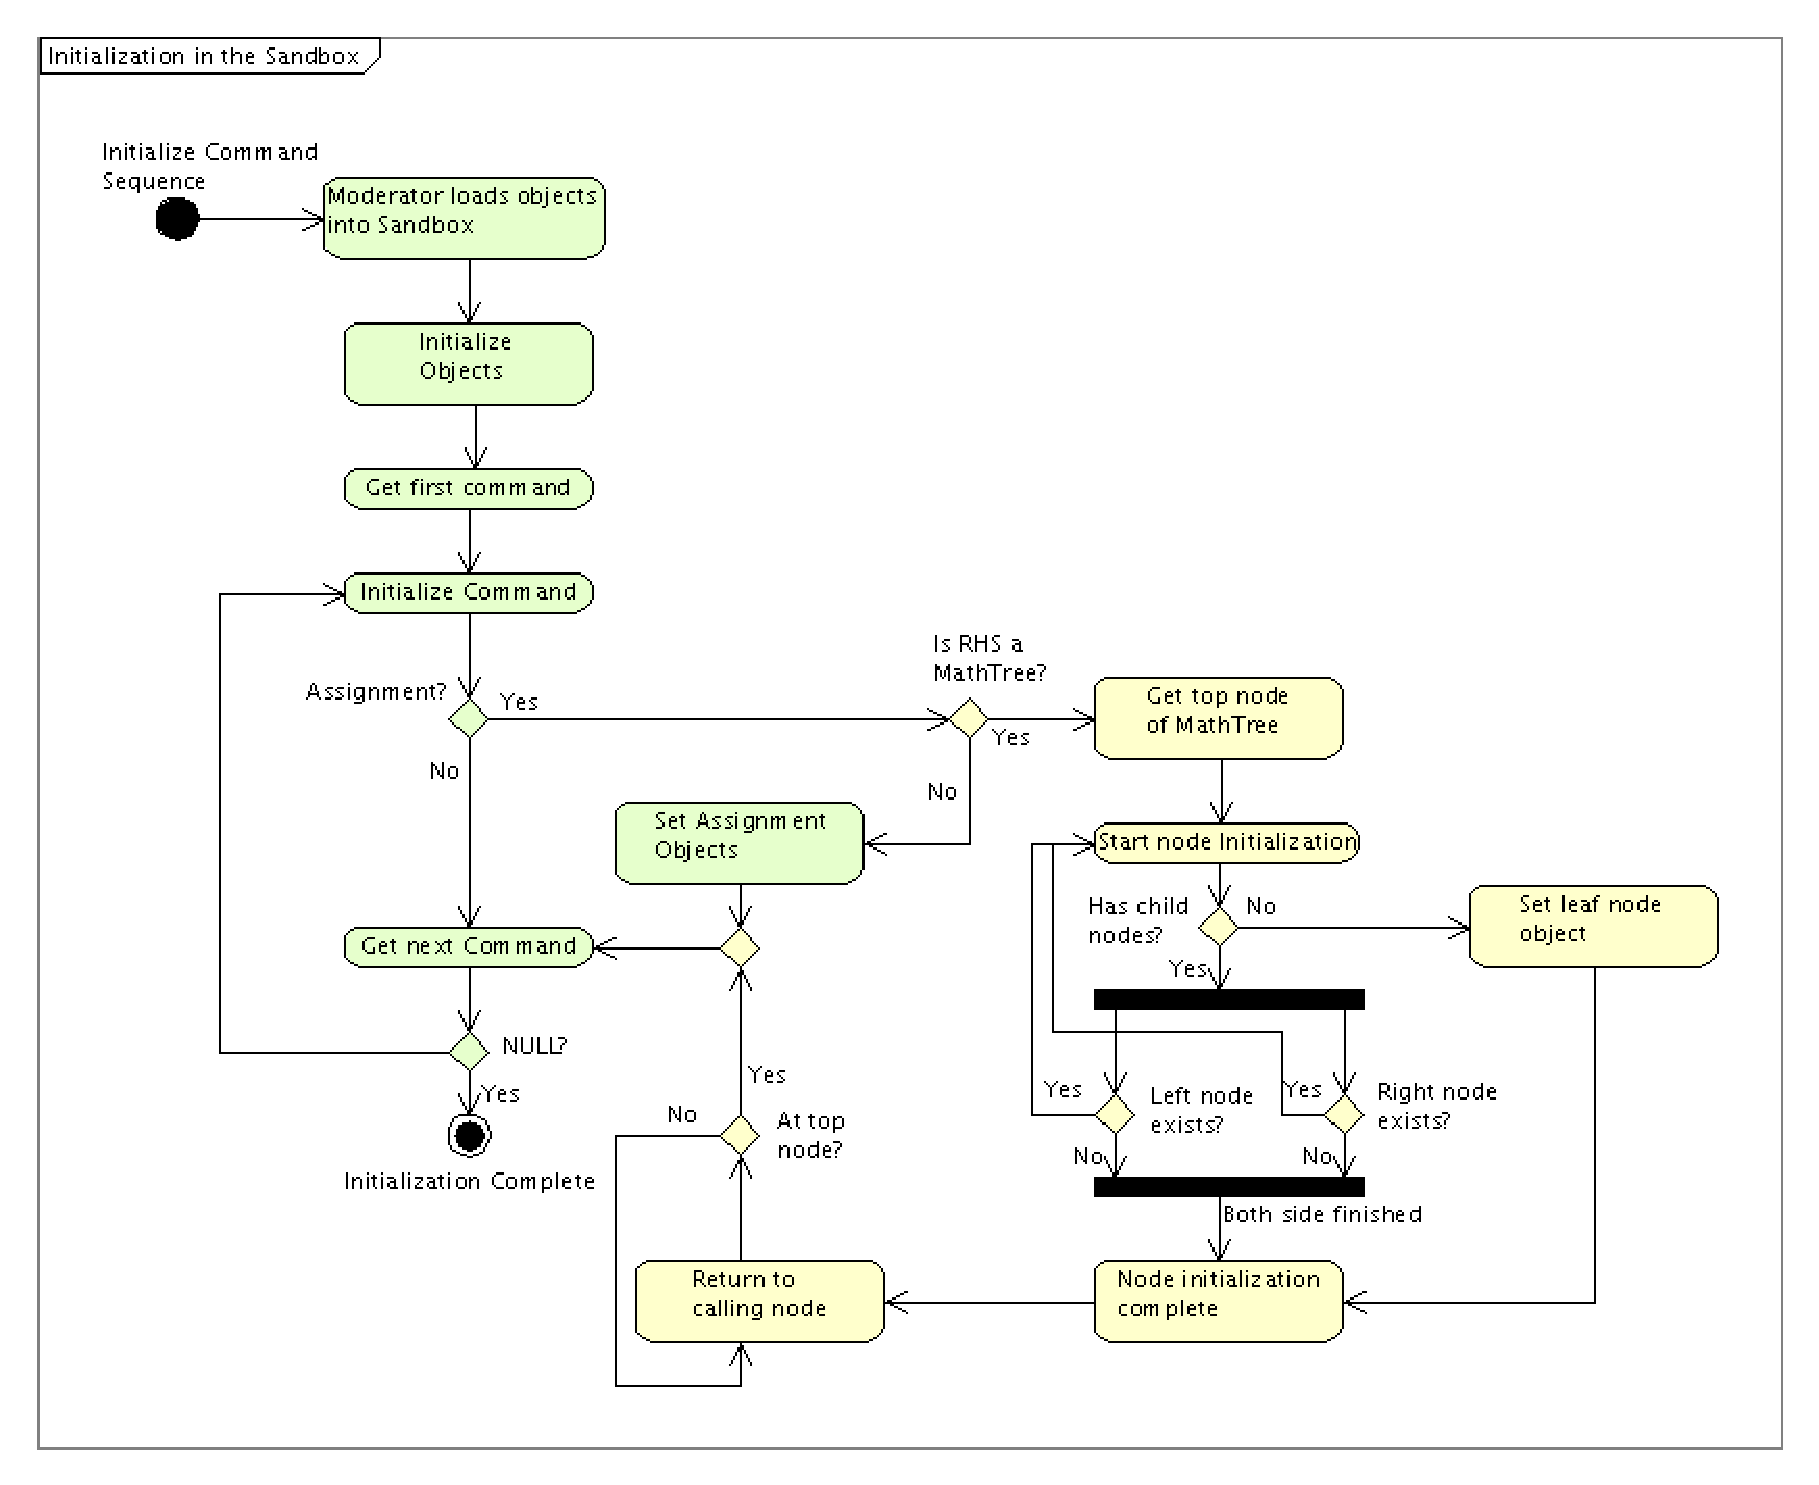
\includegraphics[scale=0.5]{Images/MathTreeInitialization.eps}
\caption{\label{figure:MathInitialization}MathTree Initialization in the
Sandbox}
\end{center}
\end{figure}

Figure~\ref{figure:MathInitialization} shows the process of initialization of
the Command Sequence in the Sandbox, with a focus on the MathTree
initialization.  Section \ref{section:SandboxInitialization} describes the
general initialization process in the Sandbox.  Sandbox initialization proceeds
as described there, initializing the objects and then the command sequence.
When the command in the sequence is an Assignment command containing in-line
mathematics, the Assignment command performs the details shown here to
initialize the MathTree.  The command first accesses the top node of the
MathTree.  If that node has subnodes, those subnodes are initialized
iteratively until a MathElement node is encountered.

When a MathElement node is encountered, that node is queried for its referenced
object's name.  If the node returns a name, that object's pointer is accessed
in the local object map owned by the Sandbox and set on the node using the
SetRefObject() method.  If the reference object name is empty, the node is a
numerical constant, and no further initialization is required.

When all of the subnodes of a MathFunction node have been initialized, that
node validates that the dimensionality of the operands are compatible with the
mathematical operation represented by the node.  This validation is done by
calling the ReportOutputs() method on the child nodes and ensuring that the
results are consistent with the requirements of the operation.  If the results
are consistent, local variables are used to save data so that parent nodes to
the current node can obtain consistency data without recursing through the
MathTree.  When the results are inconsistent with the operation, a warning
message (which indicates the inconsistency of the calculation and the text of
the line that generate the MathTree) is posted to the user, and an internal
flag is set to false, indicating that the calculation cannot be performed.
That flag is returned when the EvaluateInputs() method is called on the node.
This completes the initialization of the MathFunction node, and control is
returned to the node above the current node.

When the topmost node in the MathTree finishes initialization, the MathTree
calls the EvaluateInputs() method for the top node.  If that call returns a
false value, an exception is thrown and initialization terminates for the
Assignment command.  When the call to EvaluateInputs() succeeds, the MathTree
reports successful initialization to the Assignment command, which validates
that the result of the calculation is consistent with the object that will be
receiving the result, and, if so, returns a flag indicating that the
calculation initialized successfully.  If the resultant of the MathTree
calculation is determined to be inconsistent with the receiving object, an
exception is thrown that contains the text of the line that generated the
Assignment command, along with information about the error encountered.

\subsection{Execution}

\begin{figure}
\begin{center}
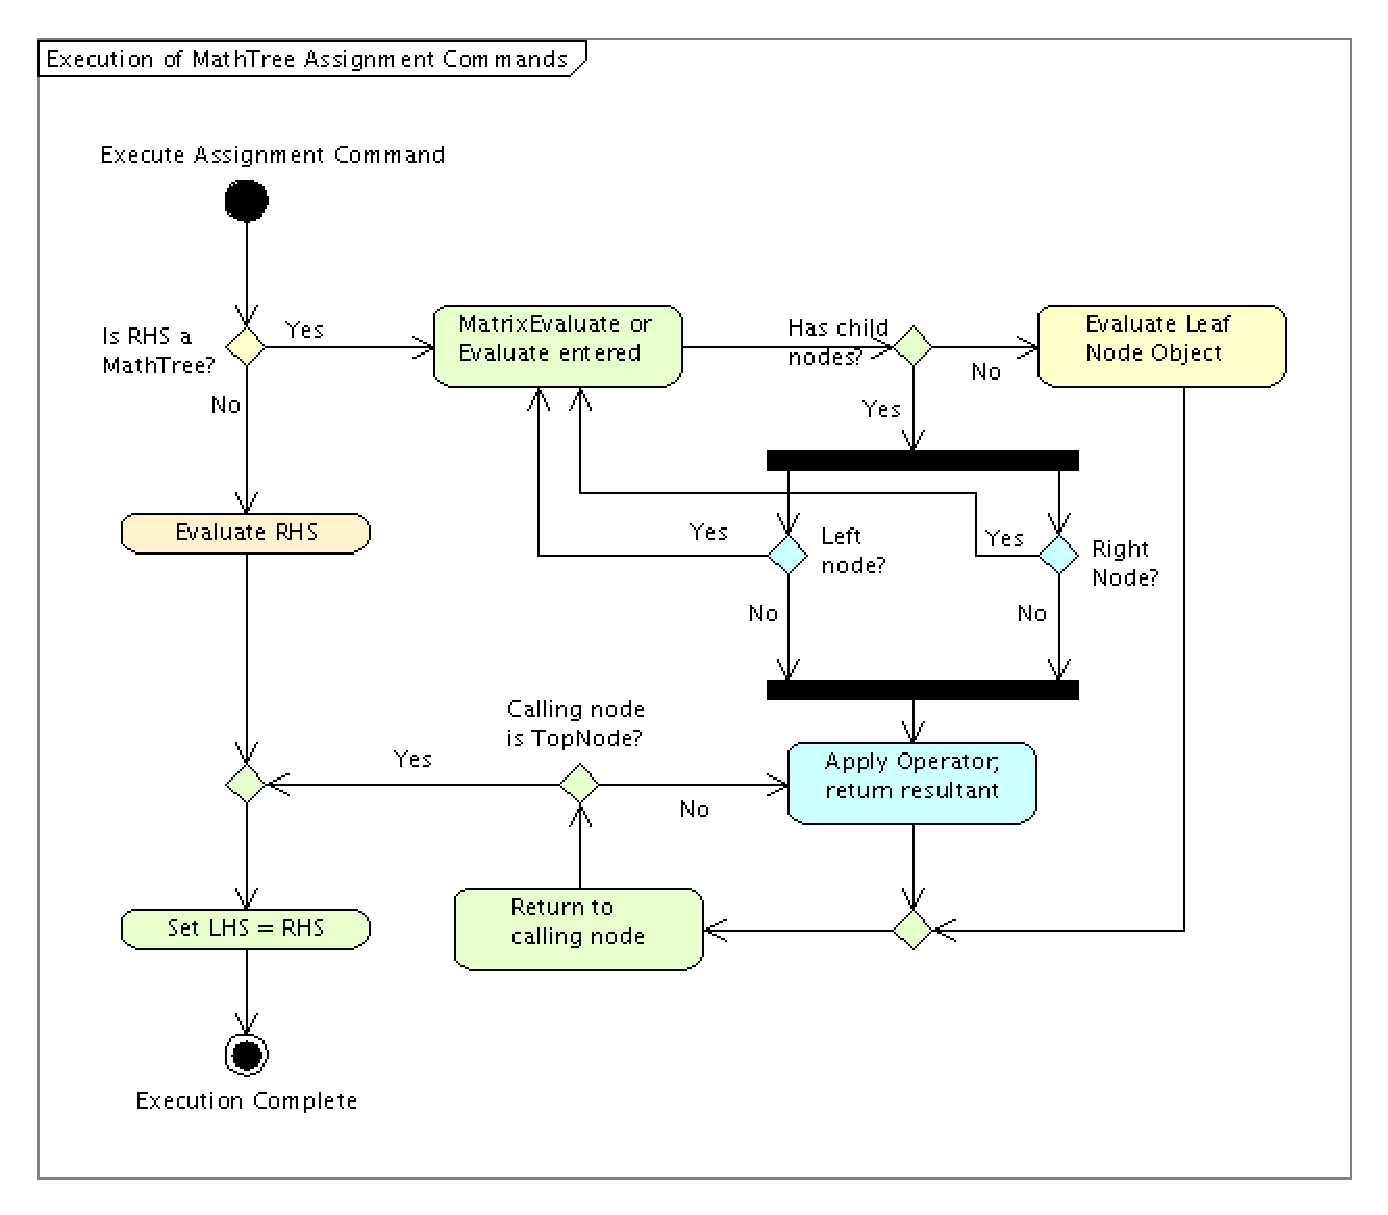
\includegraphics[scale=0.5]{Images/MathTreeExecution.eps}
\caption{\label{figure:MathTreeExecution}Evaluation of a MathTree Assignment}
\end{center}
\end{figure}

The task of evaluating a calculation is shown in Figure~\ref{figure:MathTreeExecution}.  The
Assignment command determines if a MathTree calculation is being performed by determining if the
right side of the assignment (denoted RHS in the figure) is a MathTree.  If it is, the Assignment
command checks to see if the result of the calculation should be a scalar value or a matrix by
calling ReportOutputs() on the MathTree.  If the result of this call indicates that the output is
one row by one column, the output from the calculation is scalar; otherwise, it is a matrix.  The
corresponding Evaluate() method is called on the MathTree.

The MathTree Evaluate() methods behave identically in control flow; the
difference between Evaluate() and MatrixEvaluate() is in the return value of
the call.  Similarly, the MathNode Evaluate() and MatrixEvaluate() methods
follow identical control flow, differing only in return types.  When the
correct Evaluate() method is called on the MathTree, the MathTree calls the
corresponding Evaluate() method on the topmost MathNode in the tree.
Evaluation is then performed recursively on the nodes of the tree, as described
here.

When an Evaluate() method is called on a node, the evaluation process proceeds
based on the type of node that owns the method.  If the node is a MathFunction
node, then it calls the corresponding Evaluate() method on each of its child
nodes, evaluating the left node first, then the right node.  If one of those
nodes is NULL that phase of the evaluation is skipped.  This can occur when the
mathematical operation only requires one operand -- for example, for most of
the trigonometric functions, or for unitary matrix operations like the
transpose operation.  When the child node evaluation is complete, the returned
data from that evaluation are used as the operands for the mathematical
operation.  The operation is performed, and the resulting data are passed to
the calling method.

MathElement nodes are evaluated directly when encountered, and can return
either a real number or a matrix of real numbers based on which method is
called -- either Evaluate() for a Real, or MatrixEvaluate() for a matrix.  The
result of this evaluation is passed to the calling method.  Since all of the
leaf nodes on a MathTree are MathElement nodes, these nodes terminate the
iteration through the tree.

When the calculation iteration reaches the topmost node in the MathTree, the
operation for that node is performed and the resulting data are returned to the Assignment command. 
The Assignment command then sets the data on the GMAT
object designated on the left side of the statement, designated the LHS in the
figure.  This completes the evaluation of the Assignment command.
